\documentclass{article}
\usepackage[utf8]{inputenc}
\usepackage{DASgenerator}
\usepackage{graphicx}
\usepackage{hyperref}
\usepackage{multirow}
\usepackage[table,xcdraw]{xcolor}
\usepackage{url}

%----University of Bristol Data Access Statement generator v1.2 24/10/2016----
%% DASgenerator.tex
%% Copyright 2016 University of Bristol Research Data Service
%
% This work may be distributed and/or modified under the conditions of the LaTeX Project Public License, either version 1.3 of this license or (at your option) any later version. The latest version of this license is in http://www.latex-project.org/lppl.txt and version 1.3 or later is part of all distributions of LaTeX version 2005/12/01 or later.
%
% This work has the LPPL maintenance status `maintained'.
% 
% The Current Maintainer of this work is University of Bristol Research Data Service (data-bris@bristol.ac.uk)
%
% This work consists of the files DASgenerator.sty and DASgenerator.tex

\title{Fundamentos de la Ciencia de Datos \\ PEC3: Proyectos y proyectos de datos. Ciclos y metodologías}
\author{Paula Muñoz Lago \\ paulamlago@uoc.edu \\ Master en Ciencia de Datos \\ Universitat Oberta de Catalunya}
\date{Enero 2020}



\begin{document}
\maketitle


\section{Planteamiento de un proyecto Business Intelligence o Big Data}\index{Planteamiento de un proyecto Business Intelligence o Big Data}

\subsection{Descripción y planteamiento}\index{Descripción y planteamiento}
El proyecto de Bankia "customer journey", galardonado con el premio a mejor estrategia Big data y Bussiness Intelligence de empresas españolas, recoge información de los clientes. Abarcan datos desde que comienzan a informarse sobre los servicios del banco, hasta que deja de ser cliente, pasando por su etapa en Bankia. De esta forma intentan maximizar y optimizar su experiencia y rentabilidad.

Para proceder con esta práctica, propongo un proyecto basado en el "customer journey" de Bankia. Éste consistirá en analizar el sentimiento que produce el usuario, siendo este un posible futuro cliente, ya cliente o ex-cliente. El análisis se llevará a cabo en todos los tipos de comunicación con el banco: 
\begin{itemize}
	\item Textuales: A través de la página web
	\item Por teléfono: Número de atención al cliente
	\item Presenciales: En la sucursal bancaria
\end{itemize}

El \textbf{objetivo del proyecto} será extraer el conclusiones del sentimiento que se observa en el cliente para personalizar al máximo la propuesta ofertada, de tal forma que la posibilidad de que la acepte se incremente. 

El análisis partirá de los datos extraídos del "costumer journey", en el cual se obtendrán los registros de las conversaciones e interacciones. Obteniendo los datos de cada usuario (futuro cliente, cliente o ex-cliente), además de metadatos como la hora en la que se ha mantenido dicha conversación. Otros datos a tener en cuenta será la interacción de un usuario registrado con la página web, para observar qué productos está mirando, de tal forma que si ha accedido varias veces a la página de "Depósitos bancarios", existe la posibilidad de que el individuo esté dubitativo, por lo que se le podría hacer una oferta relacionada.

Un \textbf{competidor surge} en esta fase del proyecto, y nos vemos obligados a replantear el trabajo a seguir, que se alargará por lo menos un mes y medio. Un banco de la competencia está consiguiendo nuevos clientes, dado que tiene un sistema de seguimiento del cliente mucho más certero y preciso. Se ha basado en la comunicación personal, alejándose de la comunicación cliente - máquina, como puede ser la comunicación a través de la web o con un bot telefónico. Además del seguimiento que planteamos nosotros, le han añadido la confianza en una persona y la tranquilidad que supone un asesorador que te comprenda y empatice con el cliente. Es por ello, que mantendremos nuestro objetivo de crear un sistema de Inteligencia Articifial que, una vez recogida la gran cantidad de datos del cliente, y se hayan extraído y procesado, interprete cómo se siente el cliente con respecto al banco, a la oferta propuesta o nos ayude a entender porqué lo ha dejado. Sin embargo, para adaptarnos al trato personal que triunfa en bancos de la competencia, no eliminaremos los métodos de comunicación existentes como la línea telefónica o el chat web, pero reforzaremos nuestro personal trabajando en las sucursales bancarias. Mediante un sistema de identificación del usuario en la entrada de la sucursal, accederemos a sus datos más básicos, de esta forma podremos asignarle un trabajador más acorde a su edad, para incrementar la comodidad del cliente. Además, dada la inversión en sucursales, para diversificar las comunicaciones, y no basarnos únicamente en "robots", pondremos en cada mesa un clasificador de la satisfacción del cliente. De esta forma recogeremos directamente cómo se siente tras la atención del personal de la sucursal. Deberá establecer cómo se siente, pudiendo elegir desde rojo (triste) hasta verde oscuro (feliz).

A continuación, haremos un \textbf{análisis de la gestión del cambio} según el \href{https://www.pmi.org/pmbok-guide-standards/foundational/pmbok}{PMBok (Project Management body of knowledge)}, estándar de gestión de proyectos reconocido internacionalmente.

\begin{figure}[h]
	\centering
	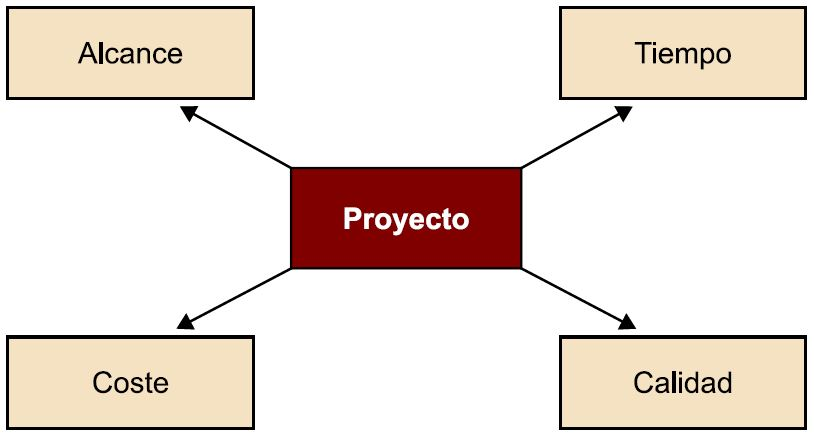
\includegraphics[scale=0.5]{PMBoK}
	\caption{Elementos críticos de la gestión de un proyecto según PMBok}
	\label{PMBoK}
\end{figure}

\subsection{Gestión del alcance}

Este área incluye los procesos necesarios para asegurar que el proyecto producirá lo que haga falta para lograr su éxito. Se identificará qué es necesario que esté incluido y qué no.

Definiremos como alcance la suma de productos, servicios y resultados que se entregarán en un proyecto. No afecta únicamente a los elementos técnicos y la documentación, también  influye en la formación, pruebas, estudios técnicos, plan de proyecto o informes de seguimiento que habrá que realizar como parte del alcance. Sin embargo, cabe diferenciar el alcance del proyecto, del alcance del producto, siendo el alcance del proyecto asociado al trabajo que hay que realizar para conseguir el producto, definido al inicio del proyecto, mientras que el alcance del segundo se centra en las características y funciones que definen un producto, servicio o resultado.

El proyecto se finalizará cuando se hayan cumplido la base del alcance, una vez producidos, validados, entregados y aceptados todos los entregables y logrados los objetivos definidos. Los pasos presentes en la gestión del alcance son los siguientes: Recopilar requisitos, definir el alcance, crear la estructura de distribución del trabajo (EDT) y verificar y realizar el control del alcance.

\subsubsection{¿Qué impacto tiene sobre el alcance?}
El cambio que debemos realizar, dado el proyecto de la competencia, hará que el alcance de nuestro proyecto \textit{vaya más allá}. No nos centraremos únicamente en saber cómo se siente el cliente para hacerle ofertas más personalizadas, también nos preocuparemos por él, para que se sienta cómodo en nuestras oficinas, y de esta forma sea más probable que acepte nuestras ofertas. Además, esta inversión en infraestructura y personal trae de la mano nuevos datos del paso del cliente por nuestra sucursal, lo cual hará que sea más sencillo la clasificación de su sentimiento.

Es por ello, que deberemos modificar el alcance realizado previamente, ya que debemos incluir la gestión de los servicios otorgados en las sucursales, así como añadir nuevas fuentes de datos en los elementos técnicos y modificar la documentación. También sería recomendable realizar un estudio para evaluar si obtendríamos mejores resultados impartiendo cursos de recursos humanos o de trato con un cliente a los empleados de la sucursal, dado el trasfondo matemático en los estudios de la mayoría de ellos. Se evaluará el gasto de dicha formación con las ganancias de la misma. Además de la instalación de la nueva fuente de datos en las sucursales, para introducir directamente cómo se ha sentido el cliente, tendremos que incluir estudios técnicos y pruebas de este nuevo sistema.

\subsubsection{¿Cómo gestionarías las posibles discrepancias con los requisitos iniciales?}

Analizaría las ganancias que los nuevos cambios acarrearían, elaborando un informe en el que explicase detalladamente cuales son los gastos de estas nuevas implementaciones, pero claramente qué ventajas nos aporta, tanto directamente al banco (como ganancias en número de clientes) como frente a la competencia, creando un sistema más moderno y robusto.

\subsubsection{¿Qué habrá que hacer con la EDT (Estructura de Desglose de Trabajo)?}

Llamamos EDT a las partes o paquetes menores de trabajo en los que se descompone cualquier proyecto. Pueden ser fases dentro de una etapa o líneas de trabajo en paralelo. De esta forma, la implementación de los cambios trae una modificación de la EDT, dados los nuevos procesos a implementar. Estos procesos son desde informáticos, incluyendo la necesidad de obtener los datos de una nueva fuente, o elaborando un sistema de identificación en la entrada de la sucursal para que los clientes sean asignados con trabajadores de características similares y así incrementar su experiencia con nuestro banco. Estas tareas pueden realizarse en paralelo, dentro del equipo informático, dado que no dependen la una de la otra. Otras tareas podrían ser la impartición de formación a los trabajadores que están \textit{cara al público} en las sucursales. Todo este tipo de sub-proyectos desglosados deberán ser incluidos en la EDT.

\subsection{Gestión del Tiempo}
Este área incluye los procesos estrictamente necesarios para asegurar que el proyecto se desarrollará según los hitos acordados con el cliente. La gestión temporal debe ser revisada y ajustada en base a cambios en otras áreas. Además de documentar el calendario o cronograma del proueceso, hay que incluir en la documentación el modelo del cronograma, añadiendo datos y criterios que se han utilizado para llegar a esas conclusiones temporales.

La gestión del tiempo del proyecto incluye los procesos siguientes: Definir, secuenciar, estimar los recursos y la duración de las actividades, además de desarrollar el cronograma y realizar el control del mismo.

\subsubsection{¿Qué utilidad tiene determinar el camino crítico cuando hay un cambio como el del enunciado?}

Siendo el camino crítico el conjunto de tareas cuyo retraso obliga a ampliar la fecha de entrega final del proyecto, es de gran utilidad a la hora de realizar cambios, intentando siempre modificar lo menos posible la espina dorsal del proyecto, el camino crítico. A la hora de aplicar estos cambios, deberían focalizarse como dependencia de alguna de sus vértebras del proyecto, evitando añadir o modificar directamente estas vértebras. Concretar un camino crítico a la hora de planificar un proyecto es de vital importancia para el seguimiento del mismo y la ubicación temporal del equipo dentro de la linea temporal hasta la finalización de éste.

\subsubsection{¿Qué harías para recuperar el posible retraso?}

Añadir recursos como contratar a más gente, con el fin de poder paralelizar taréas, o contratar recursos computacionales. En un proyecto de Inteligencia Artificial que implique, por ejemplo, redes neuronales, el entrenamiento de las mismas puede variar en función de la cantidad de datos de los que aprender, sin embargo puede llegar a tardar días. Si este incremento de recursos no fuese suficiente, y como última opción, habría que reunirse con los jefes del proyecto y evaluar la situación, con el fin de, quizás, recortar en objetivos de menor importancia, sin modificar el objetivo final del proyecto.

\subsubsection{¿Qué impacto sobre el riesgo supondría paralelizar tareas o incrementar recursos como manera de amortiguar los posibles retrasos?}

Se deben estudiar los posibles riesgos desconocidos que surgirían de la paralelización de varias tareas (\textit{fast-tracking}) para reducir el cronograma del proyecto. Si se pudiese adoptar esta medida, los riesgos a asumir serían voluntarios y podrían terminar siendo tanto positivos, como negativos.

\subsection{Gestión de los Costes}
La gestión de costes incluye los procesos relacionados con la estimación, preparación y control del presupuesto del proyecto, para que se ajuste con el aprobado.

Debido a cambios o decisiones en otras áreas, hay que ajustar el presupuesto hasta que se obtiene una propuesta coherente y según las necesidades actuales del proyecto. Sin embargo, cuando se toman dichas decisiones, también hay que tener en cuenta los costes futuros. Todo debe quedar convenientemente documentado y acordado.

La gestión de los costes del proyecto incluye los procesos: estimar costes, determinar el presupuesto y realizar el control del mismo.

\subsubsection{¿Qué impacto tendría sobre los costes del proyecto y, de haberlo, quién debería asumirlo?}

Los cambios propuestos tendrán un impacto económico en cuanto a estructuras en las sucursales, ya sea por el nuevo método de incorporación de datos, como por el sistema de identificación del cliente. Además, si se toma la decisión de formar a los trabajadores en tratamiento con el cliente o en técnicas para vender un producto, deben incluirse esos gastos también. Estos gastos debe asumirlo el propio banco, dado que el producto es para la mejora de sus propios servicios.

\subsubsection{¿Cuál es el riesgo de que haya costes no cuantificables en este momento, y de que aparezcan a la finalización del proyecto, derivados de este cambio?}

El riesgo de los gastos no cuantificables es que al finalizar el proyecto aparezca una deuda mayor que no se preveía. De esta forma, el banco puede que tarde mucho tiempo en amortizar los gastos. En cambio, al ser un riesgo, no puede acabar mal únicamente. También puede ser positivo. Al no poder cuantificar la cifra, quizás al finalizar el proyecto fuese la cifra estimada o menor. Sin embargo, este caso es menos común.

\subsubsection{¿Qué gestiones deberías realizar si el proyecto lo está desarrollando un proveedor? ¿Qué necesitarías negociar o modificar?}

Debería reunirme con el proveedor que está realizando el proyecto, y negociar quién estaría a cargo del incremento del presupuesto. Por ejemplo, si el proveedor ha tenido fallos internos, como falta de coordinación o simplemente no ha cumplido con la planificación, no negociaría un presupuesto mayor que el ya establecido, asumiendo que se han consumido las prórrogas también. Sin embargo, si se hace una propuesta de mejora, como el cambio planteado en el eljercicio, dada le presión de la competencia, en función de la economía de mi empresa, estaría totalmente dispuesta negociar la financiación de la ampliación de las características iniciales de mi proyecto.

\subsection{Gestión de Riesgos}
Un riesgo es una condición incierta que di se produce puede tener un efecto tanto negativo como positivo sobre alguna de las dimensiones del proyecto (tiempo coste alcance o calidad). La gestión de estos riesgos consiste en manejar permanentemente los riesgos potenciales o reales, siendo uno de los factores claves de la gestión.

Un riesgo puede tener una o más causas y uno o más impactos. Los riesgos positivos se denominan oportunidades, o problemas en el caso contrario. Están vinculados con elementos como hipótesis, requisitos, disponibilidad de recursos, tecnología disponible ect vinculada al proyecto. Los objetivos de la gestión de riesgos es estar preparados para enfrentarnos a ellos cuando acontezcan, para aumentar el impacto de los positivos y disminuir el de los negativos. Para ello, es recomendable disponer de políticas de procedimiento que ayuden a los directores de proyectos en el tratamiento de los riesgos. 

La gestión de riesgos incluye los siguientes procesos: planificar su gestión, identificación, realización del análisis cualitativo, cuantitativo, así como planificar las respuestas y hacer un seguimiento y control de los riesgos.

\subsubsection{¿Qué les pasa a los riesgos cuando existe un cambio?}

Los cambios en cualquier dimensión del proyecto afectan al resto de áreas en mayor o menor medida. Sin embargo, en el caso de la gestión de riesgos es mucho más relevante. Dada una modificación en cualquier otra dimensión, deben iterarse varias veces los procesos de la gestión de riesgos hasta obtener una propuesta coherente con el resto de áreas recientemente modificadas, y adecuarlo a las necesidades del proyecto. Así mismo, cuando existe una modificación en los riesgos, como la desaparición o incorporación de un riesgo, a menudo hay que revisar y ajustar el presupuesto, los recursos o el cronograma.

\subsubsection{¿Podemos identificar todos los riesgos existentes con motivo del cambio?}

Sí, uno de los riesgos podría ser la imposibilidad de implementar el sistema de identificación del usuario en las sucursales dada una falta de espacio o medios en ese edificio, entre otros. Sin embargo, debemos ser cautos a la hora de establecer riesgos, ya que la identificación de riesgos excesivos puede producir un incremento en los costes de gestión, mientras que la detección de menos riesgos de los reales puede llevar a situaciones catastróficas no previstas para el proyecto. Es por ello que, dado el cambio, se debe buscar un equilibrio entre los riesgos conocidos y desconocidos.

\subsubsection{¿Qué es un riesgo positivo?}

Un riesgo positivo es una oportunidad, como puede ser que las sucursales dispongan de más recursos de los que creíamos, o que una decisión de paralelizar tareas, que acarrea ciertos riesgos, se cumpla positivamente.


\subsection{Gestión de la Integración}
Este área de conocimiento incluye las actividades y los procesos necesarios para identificar, definir, combinar, unificar y coordinar los diferentes procesos y actividades de dirección del proyecto. Se trata de tareas de coordinación que generalmente se asocian al director del equipo. Las decisiones que tiene que tomar están relacionadas con la asignación de recursos, concreción de objetivos y la gestión de dependencias entre las partes del proyecto. Además está relacionada con la documentación y relación del proyecto con la operatoria cotidiana del cliente.

Algunos de los pasos esenciales en la gestión de la integración de un proyecto son: Desarrollar el acta de constitución, el plan de gestión, dirigir y gestionar la ejecución y hacer el seguimiento y controlar el trabajo del proyecto. También incluirá realizar el control integral de cambios y finalmente cerrar las fases o el proyecto.

\subsubsection{¿Qué ocurriría en el caso de que los procesos fundamentales del área que originan el cambio no se encuentren suficientemente formalizados y consolidados?}

Si los fundamentos del cambio no están lo suficientemente consolidados, puede derivar a una pérdida de recursos desde temporales hasta económicos. Derivaría en una mala implementación de los cambios, la cual puede pararse a mitad del proceso si se detecta la falta de formalización, o puede llegar hasta el final del proceso y detectarse en el cierre del mismo por el director del equipo. Es de vital importancia una buena formailzación de las tareas a realizar, se traten de cambios o no, para aprovechar los recursos y no tener que rehacer la planificación, como sería en el caso planteado.

\subsubsection{¿Cómo y qué argumentarías para convencer a la Dirección de retrasar la implementación de los nuevos requerimientos propuestos?}

Previa la implementación de un cambio o un requerimiento, el sistema debe ser consistente y robusto en las partes de las que dependerá el nuevo requerimiento. Es por ello que, dada esa necesidad, necesitaríamos una fase de testing para asegurarnos de la calidad del sistema anteriormente desarrollado, con el fin de ser capaces de realizar cualquier modificación antes de superponer otra tarea sobre este proceso.

\subsection{Gestión de la calidad}

Los procesos de este árrea incluyen todas las actividades que determinan políticas, objetivos y responsabilidades referentes a la calidad, para que el proyecto cumpla los objetivos fijados. Al ser el área más subjetiva, debemos diferenciar sus dimensiones a la hora de medir la calidad del producto y el proyecto; la objetiva, y la subjetiva. La primera se mide en base a unos requerimientos o estándares, mientras que la segunda se mide en lo referente a la satisfacción del cliente o su conformidad en base a sus expectativas. La calidad del producto se mide en base a sus resultados y la del proyecto en base a cómo se gestiona. Es necesario que las necesidades implícitas del cliente se transformen en requisitos mediante procesos de recopilación de requisitos, para evitar malentendidos, quejas e insatisfacción. Debemos tener presente la necesidad de encontrar un equilibro entre los procesos de calidad y las dimensiones de tiempo y costes.

La gestión de calidad incluye los procesos siguientes: Planificación, aseguramiento y control de calidad.

\subsection{Gestión de los recursos humanos}
La gestión del personal del proyecto es una de las tareas que ocupa más tiempo al director del mismo, y es crucial. Esta gestión comprende los procesos orientados a organizar, gestionar y conducir el equipo del proyecto, cuyas responsabilidades individuales pueden variar en función de las necesidades de cada momento.

La gestión de RRHH del proyecto incluye: Desarrollo del plan de RRHH, Incorporar, desarrollar y dirigir el equipo de proyectos.

\subsection{Gestión de la comunicación}
Area del conocimiento que incluye los procesos necesarios para asegurar la generación, recogida, distribución, almacenamiento, recuperación y disposición final de la información del proyecto.

Los directores de proyecto invierten una parte de su tiempo en taeras de comunicación con el cliente, con el patrocinador, el equipo, proveedores... Por ello, la mejora de las comunicaciones reduce el tiempo de estas tareas, haciéndolas más eficaces.

La gestión de la comunicación del proyecto incluye los procesos: Identificación de los interesados, planificación de las comunicaciones, distribución de la información, gestión de las expectativas de los interesados e información del rendimiento.

\subsection{Administración de compras y contratos}

Este área incluye todos los procesos y actividades que regulan las compras y contratos del proveedor con el cliente y sus diferentes socios y contratistas. La organización que administre las compras y contratos puede ser la compradora o vendedora, pero incluirá la gestión de los cambios necesarios para desarrollar o administrar el contrato. Incluyendo la administración de una posible relación con terceros.

La Administración de compras y contratos incluye: Planificación, realización, administración y clausura de las adquisiciones.

\section{Metodologías Ágiles}

El desarrollo ágil de software se basa en el \href{https://agilemanifesto.org/}{\textit{Agile Manifesto}}, que establece un conjunto de estamentos para la declaración de valores y principios que éstas metogologías deben seguir.
Algunos de esos valores son:
\begin{itemize}
\item Software funcionando sobre exhaustiva documentación
\item Personas y sus interacciones sobre herramientas y procesos
\item Colaboración con el cliente sobre negociación y contratos
\item Respuesta al cambio sobre seguir una planificación
\end{itemize}

Mientras que los 12 principios del manifiesto son los siguientes \footnote{\url{https://www.scrummanager.net/bok/index.php?title=El_manifiesto_\%C3\%A1gil}}:

\begin{enumerate}
\item Nuestra principal prioridad es satisfacer al cliente a través de la entrega temprana y continua de software de valor.
\item Son bienvenidos los requisitos cambiantes, incluso si llegan tarde al desarrollo. Los procesos ágiles se doblegan al cambio como ventaja competitiva para el cliente.
\item Entregar con frecuencia software que funcione, en periodos de un par de semanas hasta un par de meses, con preferencia en los periodos breves.
\item Las personas del negocio y los desarrolladores deben trabajar juntos de forma cotidiana a través del proyecto.
\item Construcción de proyectos en torno a individuos motivados, dándoles la oportunidad y el respaldo que necesitan y procurándoles confianza para que realicen la tarea.
\item La forma más eficiente y efectiva de comunicar información de ida y vuelta dentro de un equipo de desarrollo es mediante la conversación cara a cara.
\item El software que funciona es la principal medida del progreso.
\item Los procesos ágiles promueven el desarrollo sostenido. Los patrocinadores, desarrolladores y usuarios deben mantener un ritmo constante de forma indefinida.
\item La atención continua a la excelencia técnica enaltece la agilidad.
\item La simplicidad como arte de maximizar la cantidad de trabajo que se hace, es esencial.
\item Las mejores arquitecturas, requisitos y diseños emergen de equipos que se autoorganizan.
\item En intervalos regulares, el equipo reflexiona sobre la forma de ser más efectivo y ajusta su conducta en consecuencia.
\end{enumerate}

\subsection{¿Cómo sería el planteamiento de los cambios?}

Dado el segundo principio, no cabría duda en la implementación del cambio propuesto, al ser una ventaja competitiva para el banco. Por ello, el planteamiento de este cambio estaría orientado a las ganancias, prometiendo una entrega temprana y continua del software siempre funcionando.

Sin embargo, dada la naturaleza de este metodología, se implementaría en una única sucursal, y se harían pruebas en ella, para al tener un resultado funcionando y entregado al propio banco, extenderla al resto de forma iterativa, así como ir progresivamente ampliando su utilidad.

\subsection{¿Cuál y cómo sería el nivel de interrelación con los clientes internos?}

La relación entre los desarrolladores y el cliente será mucho más cercana si se usa esta metodología, ya que, en base al principio número 4, las personas de negocio y los desarrolladores deben trabajar juntos de forma cotidiana. De esta forma el cliente guiará en más detalle el desarrollo del producto, con el fin de reducir costes en cambios. Además, la gestión de la comunicación tendrá que cambiar, ya que se priorizará la comunicación cara a cara dentro del equipo. Sin embargo, una de las diferencias entre el agilismo y las metodologías tradicionales es que, en este caso, los desarrolladores son los expertos, y los clientes pueden aconsejar herramientas a utilizar a través de \textit{Planning poker}. Uno de los valores establece la colaboración con el cliente sobre negociación contractual, éste pone énfasis en mantener un diálogo continuo entre el equipo de desarrollo y el cliente, tan abierto y fluido como sea posible.

\subsection{¿Cómo se llevaría la planificación y la gestión del equipo externo de proyecto?}

En Agile, el equipo de personas que realiza el trabajo se autogestiona, mientras que el equipo externo, o el cliente, debe tener una jerarquía clara, para así tener los roles del cliente claros y poder relacionarnos con ellos. En el Agile Manifesto se propone avanzar de un modelo de proyecto basado en un mero contrato a un entorno colaborativo, donde éste equipo ajeno al desarrollo y el proveedor trabajen conjuntamente para alcanzar el éxito. De esta forma, el cliente debe buscar la manera de acoger a los desarrolladores, o a algunos de ellos en sus oficinas, con el fin de mejorar la comunicación y hacer más eficiente su trabajo. La empresa desarrolladora del proyecto también puede disponer de salas en las que realizar los meetings necesarios con el cliente.

\section{Metodología Clásica VS Ágil}

\subsection{¿Cuál habrías elegido y por qué?}

Hubiese escogido una metodología ágil, en concreto SCRUM \footnote{\url{https://www.scrum.org/}}, debido a que mejoran la satisfacción del cliente, dado el sistema de entrega de resultados incremental, aunque no dispongan de la funcionalidad final. Esto es, por ejemplo, si un cliente pide a una empresa la construcción de una moto, utilizando una metodología ágil en el primer \textit{sprint} o iteración la empresa entregará al cliente un monopatín, en el segundo \textit{sprint} entregará una bicicleta, para en el tercero entregar un ciclomotor y finalmente, tras las últimas indicaciones del cliente, entregar una moto. De esta forma, durante todo el proceso, el cliente observa un avance y genera confianza en el proveedor. Además, todo esto mejora la motivación del equipo, al tener objetivos a un plazo menor que en la metodología clásica, y ver el objetivo más asequible. Este sistema de objetivos a corto plazo incrementa también la eficacia a la hora de detectar problemas o errores, siendo una detección temprana. Al estar focalizados en un objetivo menos ambicioso, son más fáciles de afrontar.


\subsection{¿Podría ser cualquiera de las dos?}

Ambas metodologías plantean una forma de desarrollar software con el fin de entregarlo al cliente de la mejor forma posible. Sin embargo, adaptándonos a los tiempos que corren y observando las metodologías que siguen otras empresas, no cabe duda del rápido incremento del uso de metodologías ágiles en la última década \footnote{\url{https://marketing4ecommerce.net/la-importancia-de-implementar-la-metodologia-agile-en-una-empresa/}}. Existen varios tipos de metodologías ágiles, entre ellos Extreme Programmig, SCRUM o Kanban. Cualquiera de ellas podemos adaptarla a nuestro proyecto en la fase preeliminar. 

Dada la alta necesidad de comunicación con el cliente, y la continua posibilidad de que cambie de opinión durante el desarrollo, mantengo que las metodologías ágiles, dado su planteamiento de comunicación con éste, es la metodología más eficiente. En nuestro caso, de usar una metodología clásica, tendríamos que realizar una reunión con el cliente para recoger en una documentación (de unas 200 páginas) todos sus requerimientos (el \textit{qué}), y así elaborar otra documentación del procedimiento a seguir (el \textit{cómo}). Esto puede generar desinformación, malentendidos, y errores, al establecer una única comunicación con el cliente al principio, ya que no se le vuelve a ver hasta la entrega del producto. En nuestro caso, dado el gran número de dimensiones del proyecto, y el futuro impacto en el banco, sería una mejor opción el uso de metodologías ágiles. Además, la comunicación con el cliente no sería la única ventaja. La posibilidad de implementar los productos entregados en los diferentes \textit{sprints} haría que pudiesen probarse los productos. Se implantaría el sistema en las sucursales progresivamente, así los usuarios y trabajadores podrían ir familiarizándose con los nuevos elementos del banco antes de proceder a la implantación total del producto.

\subsection{¿Qué aspectos relativos al proyecto crees que son más decisivos para la elección de una u otra metodología de gestión?}
Como se ha comentado en el punto anterior, la necesidad de interactuar con el usuario para obtener un buen resultado, es decir, un análisis fiable de los sentimientos que emanan de su relación con el banco para poder asignarle una oferta u otra, hacen de la implantación progresiva de los nuevos elementos que deberán utilizar una buena opción. De esta manera, no saturaremos a los clientes con nuevos sistemas. No solo nos centraremos en los usuarios, como comentamos anteriormente, los trabajadores también tienen que adaptarse a los nuevos elementos tecnológicos que se irán incorporando en sus oficinas y cambiarán su forma de trabajo. Para esto ayudarán las iteraciones presentes en la metodología ágil SCRUM, mediante la cual el banco podrá integrar progesivamente los productos entregados antes de obtener el producto final.

\section{Fases del Enfoque de Implantación}

Un proyecto de BI se asimila más a un ejercicio iterativo que lineal o en cascada. Larissa Moss y Shaku Atre (2003)\footnote{\url{https://books.google.es/books/about/Business_Intelligence_Roadmap.html?id=ZV8jeV4a9_AC&redir_esc=y}} han propuesto un enfoque de implantación que ha de ajustarse a cada organización y a cada proyecto de Business Intelligence. Se compone de 7 fases, representadas en la Figura \ref{Fases}.

\begin{figure}[h]
	\centering
	\includegraphics[scale=0.7]{Fases}
	\caption{Fases del modelo propuesto por Moss y Atre(2003)}
	\label{Fases}
\end{figure}


\subsection{Fases del modelo ajustado a nuestro proyecto}

Según Larissa Moss y Shaku Atre (2003), la primera fase, \textbf{Oportunidad de negocio} consiste en evaluar la necesidad que justifica el proyecto y el nivel de \textit{readyness} para el cambio y retorno de la inversión. En nuestro caso, el \textit{business case} se basa en la positiva evaluación de ganancias bancarias en cuanto a clientes, además de las ganancias monetarias que eso conlleva, y ganancias indirectas como confianza o satisfacción de los usuarios, al entender mejor sus necesidades.

En la fase \textbf{Estrategia de soporte a las decisiones} analizamos qué datos debemos integrar, dónde almacenarlos, quién está a su cargo y qué permisos asignar a cada departamento. El resultado es un análisis de la arquitectura que se utilizará y planificación del proyecto. En nuestro caso, los ingenieros que desarrollen el sistema son los que han de tener acceso a tales datos. Si bien es cierto que mientras el sistema está en desarrollo, en la fase de testing deberán hacer pruebas con datos de ejemplo, para preservar la privacidad de los usuarios. Una vez el sistema esté implementado, los datos se irán recogiendo en una base de datos, a través de sistemas automáticos, de forma segura. Una vez el algoritmo ha procesado el estado del usuario y devuelve una respuesta, ésta aparecerá en la sesión del usuario, que únicamente pueden ver los expertos financieros que pueden ofertarle un servicio.

\textbf{Requisitos de información estratégica} se trata de saber quién toma cada decisión y qué información necesita para tomarlas. Como se ha comentado anteriormente, será un experto financiero quien, teniendo en contexto la situación del cliente, y además el sentimiento primario que presenta frente a cada servicio del que se ha informado, o que tiene o ha tenido contratado, tomará una decisión.

Como nos interesa más la situación futura que la actual, el \textbf{análisis y diseño conceptual} incluye la preparación y entrega de prototipos que funcionen tanto sobre las nuevas herramientas como en otras más sencillas como Excel. De esta forma, los datos recogidos, además de anonimizados, serán dotados con acceso al administrador del proyecto. Este podrá visualizar los datos desde las herramientas establecidas del proyecto como también descargarlo en csv o excel. Sin embargo, ya que en nuestro caso el cliente es el propio banco, no verá más resultado que el estado anímico del usuario con respecto a un cierto servicio. Y, por supuesto, el cliente podrá acceder a todos los datos que se han recogido de él si lo requiriese.

En quinto lugar, el \textbf{Diseño y construcción} establece la creación del repositorio, las ETL y el desarrollo de las diferentes capas de la aplicación sobre las herramientas del producto. También se calculará los rendimientos del sistema. En nuestro caso, será el momento en el que, si la bases de datos no está creada aún (si es la primera iteración), se creará una base de datos relacional en la que el usuario sea una clase y esté asociado con el servicio con una relación de contrato, posible contrato o ex-contrato. En iteraciones siguientes se realizará el cálculo del rendimiento, necesario para comprobar si tras el cambio implementado la eficiencia del cálculo ha mejorado o empeorado.

En la fase de testing o \textbf{Pruebas} debemos tener en cuenta que los sistemas de inteligencia de negocio se asemejan a una "caja negra". Dado que los datos y metadatos pueden no tener nada que ver con la realidad. En nuestro caso debemos realizar pruebas con un conjunto de clientes inexistentes, elaborados para todos los casos que podamos encontrar en la vida real. De esta forma reduciremos la posibilidad de fallo. En última instancia el administrador del sistema, con acceso a los datos reales, podrá hacer pruebas sobre ellos.

Finalmente debemos evaluar la \textit{release} para evaluar si se ha acertado y cumplido las expectativas y si el enfoque ha sido correcto. En nuestro caso, se puede probar el sistema con un conjunto reducido de usuarios, para comprobar si las nuevas características implementadas en el banco dan resultados positivos.

Tras todas estas fases, y como se muestra en la Figura \ref{Fases}, se vuelve a comenzar. Además se recomienda elaborar diferentes líneas de trabajo en función de los perfiles profesionales involucrados.


\subsection{CRISP-DM}

La metodología \textit{Cross Industry Standard Process for Data Mining} fue propuesta por (Chapman et al., 2000)\footnote{\url{https://www.the-modeling-agency.com/crisp-dm.pdf}}. Cubre las fases de un proyecto, sus tareas y las relaciones entre ellas. Tiene en cuenta la existencia de un cliente que no es parte del equipo desarrollador, y que el proyecto necesita un mantenimiento tras su desarrollo. El ciclo de vida de un proyecto de minería de datos consiste en seis fases mostradas en la Figura \ref{crispdm}.

\begin{figure}[h]
	\centering
	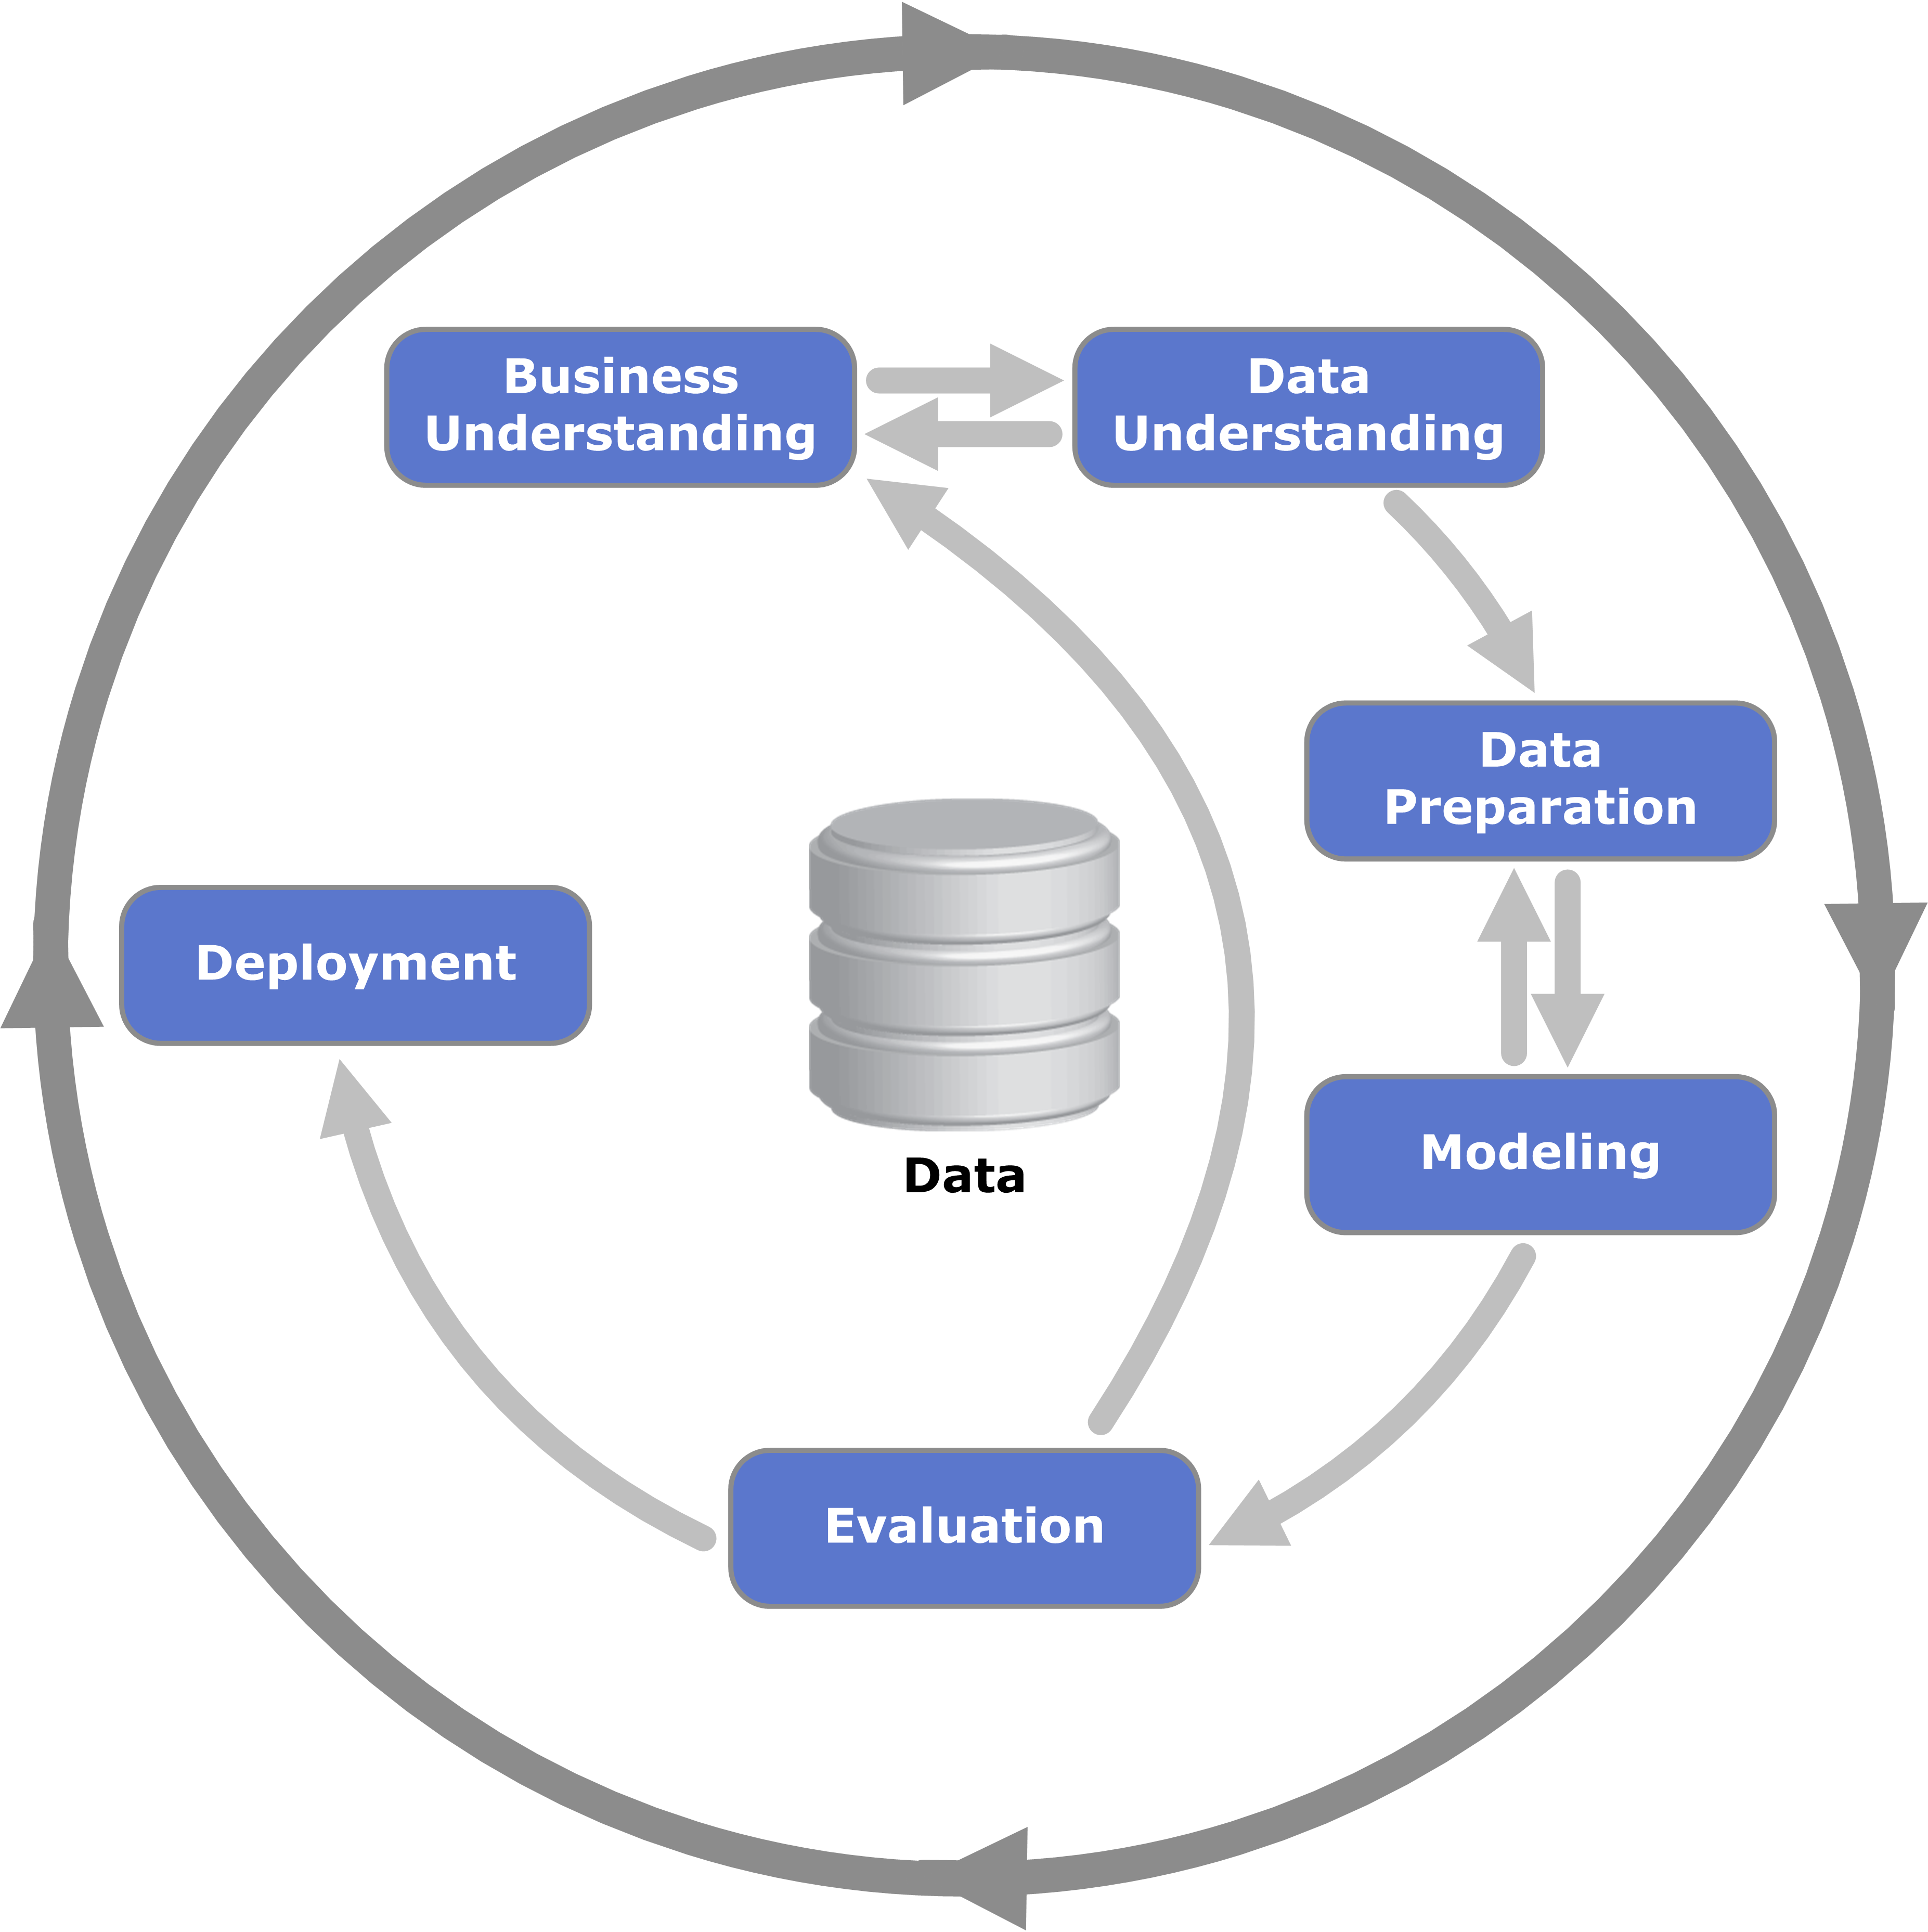
\includegraphics[scale=0.6]{CRISP-DM}
	\caption{Fases del modelo CRISP-DM}
	\label{crispdm}
\end{figure}

En primer lugar, la fase \textbf{Business Understanding} o entendimiento de negocio implica entender los objetivos del proyecto, y se elabora un plan preeliminar para conseguir los objetivos. A continuación \textbf{Estudio y comprensión de los datos} consiste en una colección de datos de prueba y ejercicios para familiarizarse con ellos. Además en esta fase se pueden descubrir subconjuntos interesantes para formar hipótesis en cuanto a información oculta. En la tercera fase, \textbf{Data preparation}, se analizan los datos y se construye el dataset final. Las tareas incluyen selección de tablas, registros, limpieza de datos, etc. La fase de \textbf{Modelado} consiste en selección y aplicación de técnicas de modelado pertinentes al problema o que se ajusten al objetivo. En quinto lugar, la fase de \textbf{Evaluación} ya parte de la construcción de uno o más modelos. Antes de proceder al despliegue final del modelo, es importante evaluarlo y revisar los pasos ejecutados para crearlo y comparar lo obtenido con los objetivos. Si los resultados obtenidos no son buenos, se inicia una nueva fase, y como muestra la Figura \ref{crispdm}, se comienza de nuevo. Sin embargo, si todo funciona correctamente, pasamos a la fase de \textbf{Puesta en producción}, incluso si el objetivo del modelo es aumentar el conocimiento de los datos, como es en nuestro caso, este conocimiento tendrá que organizarse y presentarse para que el banco pueda usarlo. \footnote{\url{https://www.sngular.com/es/data-science-crisp-dm-metodologia/}}

Dada la simplicidad de esta metodología frente a la de Larissa Moss y Shaku Atre (2003), ajustaría mi proyecto a la de Chapman et al. (2000). Una diferencia relevante es la existencia de la fase "Requisitos de información estratégica" en el primer modelo, cuya utilidad en nuestro proyecto, dadas sus características, no es clara. Además de la fase "Uso y evaluación de release", que considero mejor opción tenerlo testado sobre un conjunto de prueba y finalmente utilizarlo sobre todos los clientes, y no sobre un conjunto de los mismos, ya que podrían no aceptar a ser "conejillos de indias". De esta forma, el banco podrá hacer una campaña de marketing con su nuevo modelo de ajuste de oportunidades al cliente, así como atención al mismo en las sucursales. A su vez, CRISP-DM ofrece más flexibilidad.


\end{document}